\section{Experimento 4 segunda parte} 
Este experimento tiene como objetivo condicionar la celda de carga para que responda de manera correcta a las cargas aplicadas de manera que no se vea alterada por interferencias. Para ello, se aplicarán las cargas conocidas y se registrará la salida diferencial de la celda de carga. Se espera que después del acondicionamiento, la celda de carga muestre una respuesta a las cargas aplicadas, lo que permitirá obtener mediciones precisas.
cargas
En esta experimentación se amplificará la salida diferencial
de la celda de carga y se implementarán diferentes configuraciones que nos permitan
visualizar la susceptibilidad de nuestro circuito a las interferencias presentes tanto de
fuentes desconocidas como la generada por un motor
Se aplicara el siguiente esquema:
\begin{figure}[H]
    \centering
    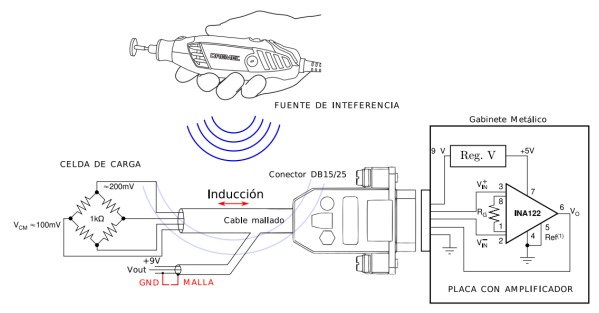
\includegraphics[width=0.5\textwidth]{images/exp4b.jpeg}
    \caption{acondicionamiento.}
    \label{fig:experimento4b}
\end{figure}
Luego de conectar la celda de carga y el amplificador de instrumentación correspondiente deberia quedar de esta forma:
\begin{figure}[H]
    \centering
    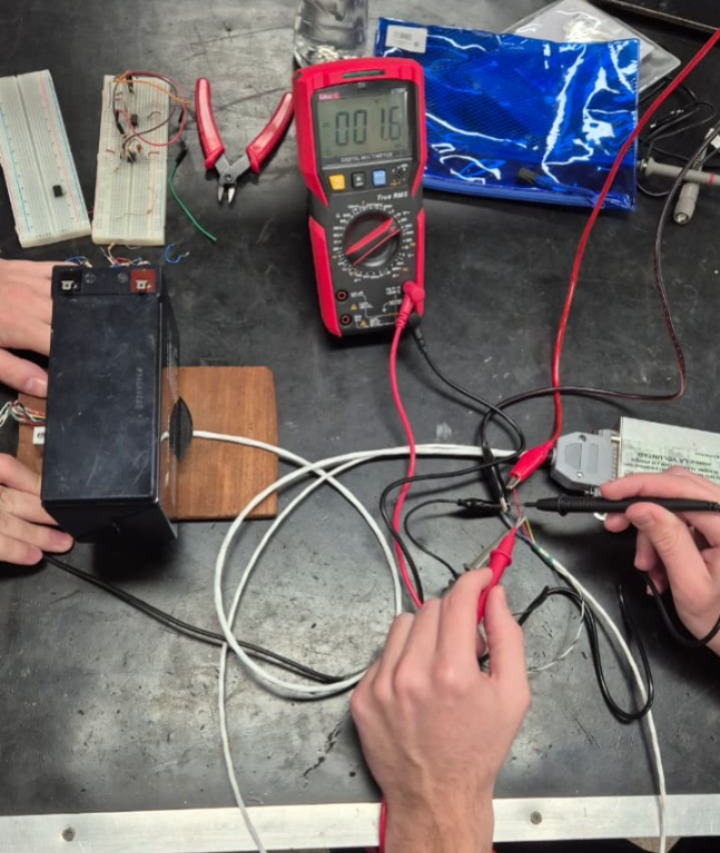
\includegraphics[width=0.5\textwidth]{images/exp4b_2.jpeg}
    \caption{acondicionamiento.}
    \label{fig:experimento4b}
\end{figure}
Con las conexiones realizadas , se procede a realizar las siguientes mediciones observando su comportamieneto en el osciloscopio correctamente configurado.Para ello se aplicará una misma carga variando la presencia del motor (encendido o apagado), el estado dela malla (acoplada y desacoplada) y la ubicacion de la placa (en el gabinete o fuera de este):
 \begin{table}[hbt!]
\centering
\begin{tabular}{ccc}
\toprule
\textbf{Placa} & \textbf{Malla} & \textbf{Motor (gen. interferencia)} \\
\cmidrule(lr){1-1} \cmidrule(lr){2-2} \cmidrule(lr){3-3}
\rowcolor{black!10} en gabinete & unida a GND & apagado \\
en gabinete & unida a GND & encendido \\
\rowcolor{black!10} en gabinete & desacoplada & apagado \\
en gabinete & desacoplada & encendido \\
\rowcolor{black!10} fuera de gabinete & desacoplada & apagado \\
fuera en gabinete & desacoplada & encendido \\
\bottomrule
\end{tabular}
\end{table}
\begin{figure}[H]
    \centering
    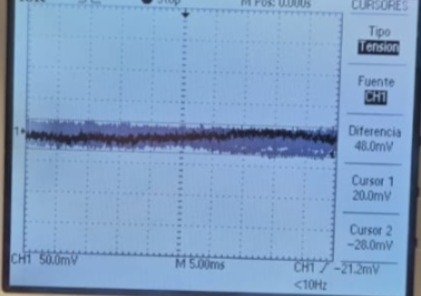
\includegraphics[width=0.425\textwidth]{images/acopladosinruido.jpeg}
    \caption{Celda de carga acoplada sin ruido.}
    \label{fig:experimento4b_1}

    \vspace{0.3cm}

    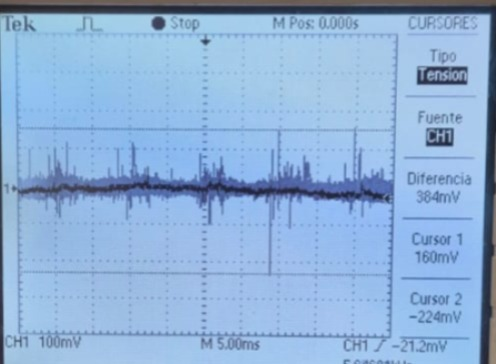
\includegraphics[width=0.425\textwidth]{images/acopladoruido.jpeg}
    \caption{Celda de carga acoplada con ruido.}
    \label{fig:experimento4b_2}

    \vspace{0.3cm}

    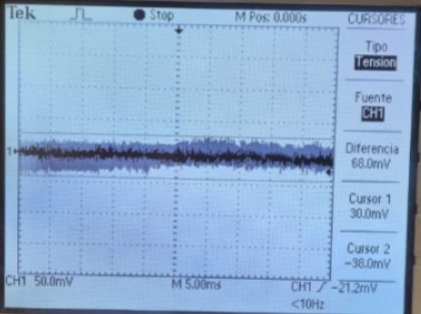
\includegraphics[width=0.425\textwidth]{images/desacopladosinruido.jpeg}
    \caption{Celda de carga desacoplada sin ruido.}
    \label{fig:experimento4b_3}
\end{figure}

\begin{figure}[H]
    \centering
    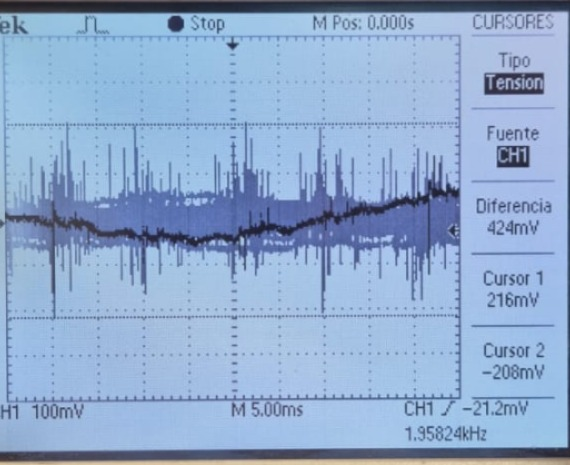
\includegraphics[width=0.425\textwidth]{images/desacopladoruido.jpeg}
    \caption{Celda de carga desacoplada con ruido.}
    \label{fig:experimento4b_4}

    \vspace{0.3cm}

    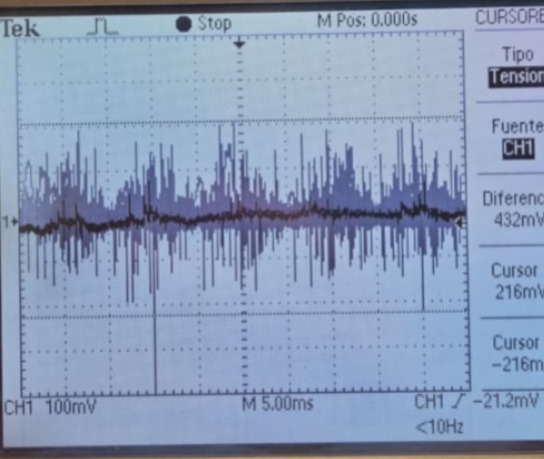
\includegraphics[width=0.4\textwidth]{images/fueraconmotor.jpeg}
    \caption{Celda de carga fuera del gabinete con motor encendido.}
    \label{fig:experimento4b_5}

    \vspace{0.3cm}

    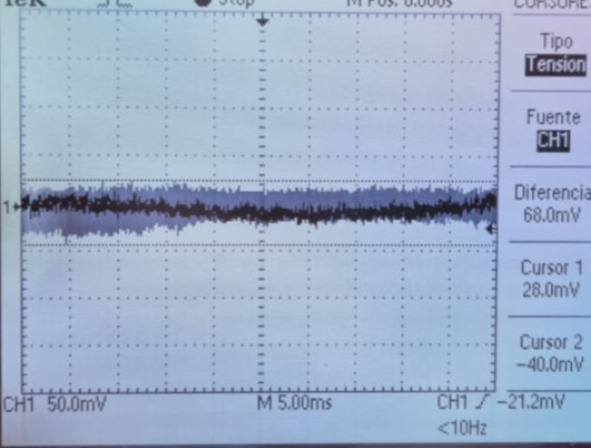
\includegraphics[width=0.4\textwidth]{images/fuerasinmotor.jpeg}
    \caption{Celda de carga fuera del gabinete sin motor.}
    \label{fig:experimento4b_6}
\end{figure}



